Konstruieren Sie einen Pushdown-Automaten, der die durch folgende
Grammatik definierte Sprache akzeptiert:
\begin{align*}
S&\rightarrow \varepsilon\\
 &\rightarrow SS\\
 &\rightarrow KSV\\
 &\rightarrow VSK\\
K&\rightarrow 
\text{\tt b}\,|\,
\text{\tt c}\,|\,
\text{\tt d}\,|\,
\text{\tt f}\,|\,
\text{\tt g}\,|\,
\text{\tt h}\,|\,
\text{\tt j}\,|\,
\text{\tt k}\,|\,
\text{\tt l}\,|\,
\text{\tt m}\,|\,
\text{\tt n}\,|\,
\text{\tt p}\,|\,
\text{\tt q}\,|\,
\text{\tt r}\,|\,
\text{\tt s}\,|\,
\text{\tt t}\,|\,
\text{\tt v}\,|\,
\text{\tt w}\,|\,
\text{\tt x}\,|\,
\text{\tt y}\,|\,
\text{\tt z}
\\
V&\rightarrow
\text{\tt a}\,|\,
\text{\tt e}\,|\,
\text{\tt i}\,|\,
\text{\tt o}\,|\,
\text{\tt u}
\end{align*}
Zeigen Sie, dass das Wort {\tt freude} zwei verschiedene
parse trees hat.

\thema{Stackautomat}
\thema{eindeutiger Parse Tree}

\begin{loesung}
Die Sprache enthält die Wörter
\[
\varepsilon,
\text{\it KV},
\text{\it VK},
\text{\it VVKK},
\text{\it VKVK},
\text{\it KVKV},
\text{\it KKVV},\dots
\]
also alle Wörter, die gleich viele Konsonanten wie Vokale enthalten.
Wir brauchen also nur einen Pushdown-Automaten, der feststellen kann,
ob die gleiche Anzahl Vokale wie Konsonanten gelesen worden sind. Dazu
verwenden wir als Stackalphabet $\Gamma = \{{\tt \$}, {\tt +}\}$,
wobei die {\tt +} einen "Uberschuss von Konsonanten oder Vokalen
anzeigen. Welches Zeichen gerade im "Uberfluss vorhanden ist,
zeigt der aktuelle Zustand, der entweder $V$ ("Uberschuss an
Vokalen) oder $K$ ("Uberschuss an Konsonanten) sein kann.
Der Automat ist im Zustand $Z$, wenn gleich viele Vokale wie
Konsonanten gelesen wurden:
\begin{center}
\begin{tikzpicture}[>=latex,thick]
\def\zustand#1#2{
	\node at #1 {#2};
	\draw #1 circle[radius=0.4];
}
\def\akzeptierzustand#1#2{
	\zustand{#1}{#2}
	\draw #1 circle[radius=0.35];
}
\coordinate (s) at (-2,3);
\coordinate (S) at (0,3);
\coordinate (V) at (-3,0);
\coordinate (Z) at (0,0);
\coordinate (K) at (3,0);
\coordinate (E) at (0,-3);
\zustand{(S)}{$S$}
\zustand{(V)}{$V$}
\zustand{(Z)}{$Z$}
\zustand{(K)}{$K$}
\akzeptierzustand{(E)}{$E$}
\draw[->,shorten >= 0.4cm,shorten <= 0.4cm] (s) -- (S);
\draw[->,shorten >= 0.4cm,shorten <= 0.4cm] (S) -- (Z);
\draw[->,shorten >= 0.4cm,shorten <= 0.4cm] (Z) -- (E);
\node at ($0.6*(S)+0.4*(Z)$)
	[right] {$\varepsilon,\varepsilon\to\texttt{\$}$\strut};
\node at ($0.4*(Z)+0.6*(E)$)
	[right] {$\varepsilon,\texttt{\$}\to\varepsilon$\strut};
\draw[->,shorten >= 0.4cm,shorten <= 0.4cm]
	(K) to[out=20,in=70,distance=1.4cm] (K);
\draw[->,shorten >= 0.4cm,shorten <= 0.4cm]
	(K) to[out=-20,in=-70,distance=1.4cm] (K);
\draw[->,shorten >= 0.4cm,shorten <= 0.4cm]
	(V) to[out=150,in=110,distance=1.4cm] (V);
\draw[->,shorten >= 0.4cm,shorten <= 0.4cm]
	(V) to[out=-150,in=-110,distance=1.4cm] (V);
\draw[->,shorten >= 0.4cm,shorten <= 0.4cm]
	(Z) to[out=20,in=160] (K);
\draw[->,shorten >= 0.4cm,shorten <= 0.4cm]
	(K) to[out=-160,in=-20] (Z);
\draw[->,shorten >= 0.4cm,shorten <= 0.4cm]
	(Z) to[out=160,in=20] (V);
\draw[->,shorten >= 0.4cm,shorten <= 0.4cm]
	(V) to[out=-20,in=-160] (Z);
\node at ($0.5*(V)+0.5*(Z)+(0,0.6)$) {$V,\varepsilon\to\texttt{+}$\strut};
\node at ($0.5*(K)+0.5*(Z)+(0,0.6)$) {$K,\varepsilon\to\texttt{+}$\strut};
\node at ($0.5*(V)+0.5*(Z)+(0,-0.6)$)
	{$\varepsilon,\texttt{\$}\to\texttt{\$}$\strut};
\node at ($0.5*(K)+0.5*(Z)+(0,-0.6)$)
	{$\varepsilon,\texttt{\$}\to\texttt{\$}$\strut};
\node at ($(V)+(-0.7,0.7)$) [left] {$V,\varepsilon\to\texttt{+}$\strut};
\node at ($(K)+(0.7,0.7)$) [right] {$K,\varepsilon\to\texttt{+}$\strut};
\node at ($(V)+(-0.7,-0.7)$) [left] {$K,\texttt{+}\to\varepsilon$\strut};
\node at ($(K)+(0.7,-0.7)$) [right] {$V,\texttt{+}\to\varepsilon$\strut};
\end{tikzpicture}
\end{center}
%\[
%\entrymodifiers={++[o][F]}
%\xymatrix @+10mm {
%*+\txt{}\ar[r]
%        &{s}\ar[d]^{\varepsilon,\varepsilon\to{\tt \$}}
%\\
%{V} \ar@(ul,dl)_{\scriptsize    \begin{gathered}
%                                        V,\varepsilon\to {\tt +}\\
%                                        K,{\tt +}\to\varepsilon
%                                \end{gathered}}
%    \ar@/_/[r]_{\varepsilon,{\tt \$}\to{\tt \$}}
%        &{Z} \ar@/^/[r]^{K,\varepsilon\to {\tt +}}
%             \ar@/_/[l]_{V,\varepsilon\to {\tt +}}
%             \ar[d]^{\varepsilon,{\tt\$}\to\varepsilon}
%                &{K} \ar@(ur,dr)^{\scriptsize   \begin{gathered}
%                                                        K,\varepsilon\to {\tt +}\\
%                                                        V,{\tt +}\to\varepsilon
%                                                \end{gathered}}
%                     \ar@/^/[l]^{\varepsilon,{\tt \$}\to{\tt\$}}
%\\
%*+\txt{}
%        &*++[o][F=]{E}
%}
%\]
Dabei stehen die Variablen $V$ und $K$ in den Übergängen für 
die Terminalsymbole, in die sie gemäss der Regeln der Grammatik
verwandelt werden können.

Die möglichen Parse Trees sind:
\begin{center}
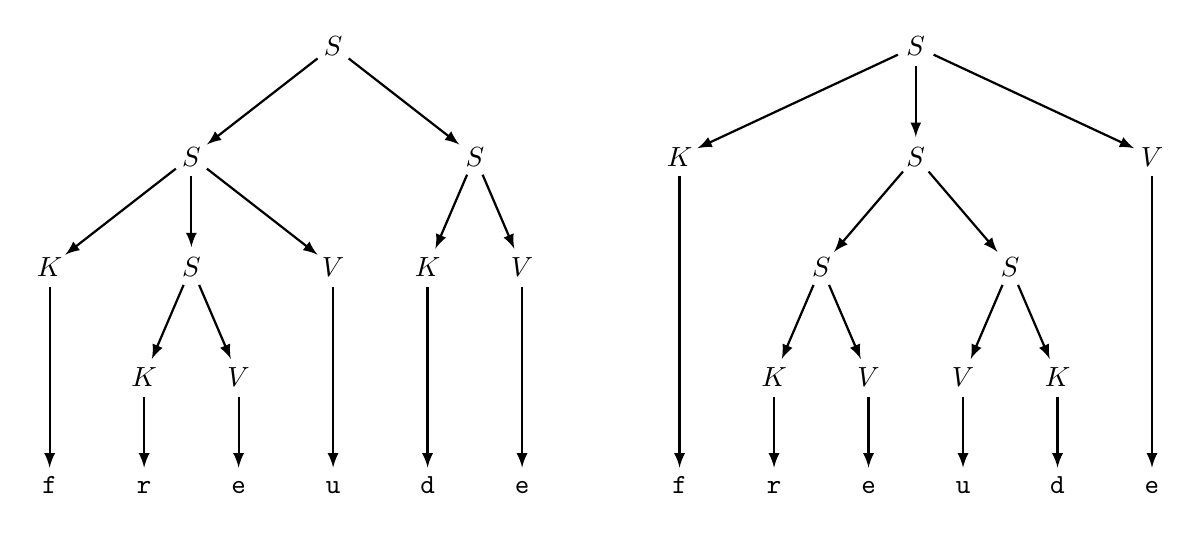
\begin{tikzpicture}[>=latex,thick]
\def\l{1.2}
\def\s{1.4}
\begin{scope}
\coordinate (s1) at ({\l},0);
\coordinate (s2) at ({-0.5*\l},{-\s});
\coordinate (s3) at ({2.5*\l},{-\s});
\coordinate (k1) at ({-2*\l},{-2*\s});
\coordinate (s4) at ({-0.5*\l},{-2*\s});
\coordinate (v1) at ({\l},{-2*\s});
\coordinate (k2) at ({2*\l},{-2*\s});
\coordinate (v2) at ({3*\l},{-2*\s});
\coordinate (k3) at ({-1*\l},{-3*\s});
\coordinate (v3) at (0,{-3*\s});
\coordinate (w1) at ({-2*\l},{-4*\s});
\coordinate (w2) at ({-1*\l},{-4*\s});
\coordinate (w3) at (0,{-4*\s});
\coordinate (w4) at ({1*\l},{-4*\s});
\coordinate (w5) at ({2*\l},{-4*\s});
\coordinate (w6) at ({3*\l},{-4*\s});
\node at (s1) {$S$};
\node at (s2) {$S$};
\node at (s3) {$S$};
\node at (s4) {$S$};
\node at (k1) {$K$};
\node at (k2) {$K$};
\node at (k3) {$K$};
\node at (v1) {$V$};
\node at (v2) {$V$};
\node at (v3) {$V$};
\node at (w1) {\texttt{f}\strut};
\node at (w2) {\texttt{r}\strut};
\node at (w3) {\texttt{e}\strut};
\node at (w4) {\texttt{u}\strut};
\node at (w5) {\texttt{d}\strut};
\node at (w6) {\texttt{e}\strut};
\draw[->,shorten >= 0.25cm,shorten <= 0.25cm] (s1) -- (s2);
\draw[->,shorten >= 0.25cm,shorten <= 0.25cm] (s1) -- (s3);
\draw[->,shorten >= 0.25cm,shorten <= 0.25cm] (s2) -- (k1);
\draw[->,shorten >= 0.25cm,shorten <= 0.25cm] (s2) -- (s4);
\draw[->,shorten >= 0.25cm,shorten <= 0.25cm] (s2) -- (v1);
\draw[->,shorten >= 0.25cm,shorten <= 0.25cm] (s4) -- (k3);
\draw[->,shorten >= 0.25cm,shorten <= 0.25cm] (s4) -- (v3);
\draw[->,shorten >= 0.25cm,shorten <= 0.25cm] (s3) -- (k2);
\draw[->,shorten >= 0.25cm,shorten <= 0.25cm] (s3) -- (v2);
\draw[->,shorten >= 0.25cm,shorten <= 0.25cm] (k1) -- (w1);
\draw[->,shorten >= 0.25cm,shorten <= 0.25cm] (k3) -- (w2);
\draw[->,shorten >= 0.25cm,shorten <= 0.25cm] (v3) -- (w3);
\draw[->,shorten >= 0.25cm,shorten <= 0.25cm] (v1) -- (w4);
\draw[->,shorten >= 0.25cm,shorten <= 0.25cm] (k2) -- (w5);
\draw[->,shorten >= 0.25cm,shorten <= 0.25cm] (v2) -- (w6);
\end{scope}
\begin{scope}[xshift=8cm]
\coordinate (s1) at ({0.5*\l},0);
\coordinate (k1) at ({-2*\l},{-\s});
\coordinate (s2) at ({0.5*\l},{-\s});
\coordinate (v1) at ({3*\l},{-\s});
\coordinate (s3) at ({-0.5*\l},{-2*\s});
\coordinate (s4) at ({1.5*\l},{-2*\s});
\coordinate (k2) at ({-1*\l},{-3*\s});
\coordinate (v2) at ({0*\l},{-3*\s});
\coordinate (v3) at ({1*\l},{-3*\s});
\coordinate (k3) at ({2*\l},{-3*\s});
\coordinate (w1) at ({-2*\l},{-4*\s});
\coordinate (w2) at ({-1*\l},{-4*\s});
\coordinate (w3) at ({0*\l},{-4*\s});
\coordinate (w4) at ({1*\l},{-4*\s});
\coordinate (w5) at ({2*\l},{-4*\s});
\coordinate (w6) at ({3*\l},{-4*\s});
\node at (s1) {$S$};
\node at (s2) {$S$};
\node at (s3) {$S$};
\node at (s4) {$S$};
\node at (v1) {$V$};
\node at (v2) {$V$};
\node at (v3) {$V$};
\node at (k1) {$K$};
\node at (k2) {$K$};
\node at (k3) {$K$};
\node at (w1) {\texttt{f}\strut};
\node at (w2) {\texttt{r}\strut};
\node at (w3) {\texttt{e}\strut};
\node at (w4) {\texttt{u}\strut};
\node at (w5) {\texttt{d}\strut};
\node at (w6) {\texttt{e}\strut};
\draw[->,shorten >= 0.25cm,shorten <= 0.25cm] (s1) -- (s2);
\draw[->,shorten >= 0.25cm,shorten <= 0.25cm] (s1) -- (k1);
\draw[->,shorten >= 0.25cm,shorten <= 0.25cm] (s1) -- (v1);
\draw[->,shorten >= 0.25cm,shorten <= 0.25cm] (s2) -- (s3);
\draw[->,shorten >= 0.25cm,shorten <= 0.25cm] (s2) -- (s4);
\draw[->,shorten >= 0.25cm,shorten <= 0.25cm] (s3) -- (k2);
\draw[->,shorten >= 0.25cm,shorten <= 0.25cm] (s3) -- (v2);
\draw[->,shorten >= 0.25cm,shorten <= 0.25cm] (s4) -- (k3);
\draw[->,shorten >= 0.25cm,shorten <= 0.25cm] (s4) -- (v3);
\draw[->,shorten >= 0.25cm,shorten <= 0.25cm] (k1) -- (w1);
\draw[->,shorten >= 0.25cm,shorten <= 0.25cm] (k2) -- (w2);
\draw[->,shorten >= 0.25cm,shorten <= 0.25cm] (v2) -- (w3);
\draw[->,shorten >= 0.25cm,shorten <= 0.25cm] (v3) -- (w4);
\draw[->,shorten >= 0.25cm,shorten <= 0.25cm] (k3) -- (w5);
\draw[->,shorten >= 0.25cm,shorten <= 0.25cm] (v1) -- (w6);
\end{scope}
\end{tikzpicture}
\end{center}
%\[
%\xymatrix{
%        &
%                &S\ar[dl] \ar[drr]
%\\
%        &S\ar[dl] \ar[d] \ar[drr]
%                &
%                        &
%                                &S\ar[d] \ar[dr]
%\\
%K\ar[dd]
%        &S\ar[d] \ar[dr]
%                &
%                        &V\ar[dd]
%                                &K\ar[dd]
%					&V\ar[dd]
%\\
%	&K\ar[d]
%		&V\ar[d]
%			&
%				&
%					&
%\\
%{\tt f}
%        &{\tt r}
%                &{\tt e}
%                        &{\tt u}
%                                &{\tt d}
%                                        &{\tt e}
%}
%\]
%
%\[
%\xymatrix{
%        &
%                &S\ar[dll] \ar[d] \ar[drrr]
%\\
%K\ar[ddd]
%        &
%                &S\ar[dl] \ar[dr]
%                        &
%                                &
%                                        &V\ar[ddd]
%\\
%        &S\ar[d] \ar[dr]
%                &
%                        &S\ar[d] \ar[dr]
%                                &
%\\
%	&K\ar[d]
%		&V\ar[d]
%			&V\ar[d]
%				&K\ar[d]
%					&
%\\
%{\tt f}
%        &{\tt r}
%                &{\tt e}
%                        &{\tt u}
%                                &{\tt d}
%                                        &{\tt e}
%}
%\]
Darin haben wir zur Abkürzung die Produktionsregeln
$S\to KV$ und $S\to VK$ verwendet, welche sich durch
zusammensetzen von $S\to KSV$ bzw.~$S\to VSK$ mit $S\to\varepsilon$
ergeben.
\end{loesung}
